%Para IEEE usar la siguiente línea
%IEEE
%\documentclass[conference]{./sty/IEEEtran}
%Springer
\documentclass{./sty/llncs}
\newcommand{\head}[1]{\textnormal{\textbf{#1}}}
\usepackage[utf8]{inputenc}
\usepackage{graphicx}
\usepackage{array}
% correct bad hyphenation here
\hyphenation{op-tical net-works semi-conduc-tor}
\begin{document}
\graphicspath{images/}
%\title{Hacia la incorporación de Consciencia Contextual en Sistemas Colaborativos Móviles} 

\title{Towards Incorporating Contextual Awareness in Collaborative Video Games}
%\title{}
%\author{}
%\institute{}

%\author{Luis G. Montané-Jiménez \and Edgard Benítez-Guerrero \and Carmen Mezura-Godoy. \email{lmontane@uv.mx \and edbenitez@uv.mx \and cmezura@uv.mx}}
%\institute{Factultad de Estadística e Informática, Universidad Veracruzana, Xalapa 91020, México.}
% make the title area
\maketitle

\begin{abstract} 
%\boldmath
Context-Aware Groupware Systems (CAGS) allow building more dynamics environments in order to help users to have a better performance in collaborative activities. The CAGS could be present in multiple domains (e.g. entertainment, hospitals, tourism, etc.), particularly in the entertainment, the Video Games are a current topic of interest. The technological advance brings new mechanisms which could be used to improve the computer-mediated collaboration. In traditional Collaborative First-Persons-Shooter video games (FPS), the collaboration means provided to the users are traditionally text messages, audio messages or predefined audio messages, which due to the velocity of the FPS games are not sufficient for that the users effectively collaborate. 

\keywords{CSCW, Videogames, Groupware}

\end{abstract}
% no keywords
\section{Introduction}
\label{sec:intro}
Para la construcción de Sistemas Colaborativos Conscientes del Contexto existen dos áreas directamente involucradas, por una parte se encuentra el Computer Supported Cooperative Work (CSCW) abordando los aspectos relacionados a la colaboración entre las personas mediante el uso de la tecnología, y por otra parte la Conscienca Contextual, contemplando aspectos de detección, administración y uso del contexto para proveer aplicaciones más dinámicas y versátiles que satisfagan de mejor manera las necesidades de los usuarios. Aunque las dos áreas se encargan de estudiar por separado dichos tópicos, existe un punto donde las áreas se únen y combinan con el fin de implementar Context-Aware Groupware Systems (CAGS). En la figura \ref{fig:contextoInvestigacion} se resumen las áreas involucradas en el presente trabajo de investigación, mostrando cronológicamente los enfoques y trabajos que han surgido a lo largo de los últimos años. 

\begin{table}[htbp]
%\renewcommand{\arraystretch}{1.2}
%\normalsize
	\centering
	\begin{tabular}{ll}
			\hline
		 	Category & Indicators \\
			\hline
			 Affective & Expression of emotions, Use of humor, Self-disclosure.   \\
			 Interactive &  Continuing a thread, Quoting from other messages,   \\
			 & Referring explicity  to other's messages, Asking questions, \\
			 & Complimenting expressing appreciation, Expressing agreement.   \\
			 Cohesive & Vocatives, Addresses or refers to the group using inclusive \\
			 & pronouns, Phatics, salutations. \\
			\hline	 
	\end{tabular}
	\caption{Categories of social presence.}
	\label{tab:socialPresence}
\end{table}

This paper presents a review of the current points of view that exist for the development of CAGS, taken from the perspective of emerging technologies in CSCW. This document is structured this way: section \ref{sec:review} describes a review of the CAGS, section \ref{sec:videogame} describes the tendency of Collaborative Videogame Systems, afterwards, section \ref{sec:study} describes the experimental study where the experiments were performed, section \ref{sec:results} describes about the obtained results from the experiments, section \ref{sec:discussion} we discuss the results and finally, section \ref{sec:conclusion} presents conclusions and future works.

%Generalidades de los Sistemas Colaborativos Conscientes del Contexto
\section{Review of Context-Aware Groupware Systems} 
\label{sec:review}
Following a review of the state of the art is made for i) Groupware Systems, ii) Context-Aware Systems and iii) Context-Aware Groupware Systems. Figure \ref{fig:contextoInvestigacion} summarizes the areas involved in the present research, showing the approaches and related work emerged over the few last years.

\subsection{Groupware Systems}

For the definition of human activities social and cultural aspects have been studied for over a decade, from general approaches as \textit{theories} \cite{Engestrom87} and \textit{models} \cite{Mezura03,Fitzpatrick03,Martel06}, to more specific approaches such as \textit{frameworks}, \textit{architectures} or \textit{systems} \cite{Preguica05,Guicking06}. These studies have been useful to represent and describe the elements and relations involved, which are relevant in traditional collaborative activities. However, there is still exploring, designing and evaluating new approaches that help in creating next-generation Groupware Systems (GS).

\begin{figure}[ht!]
	\centering
	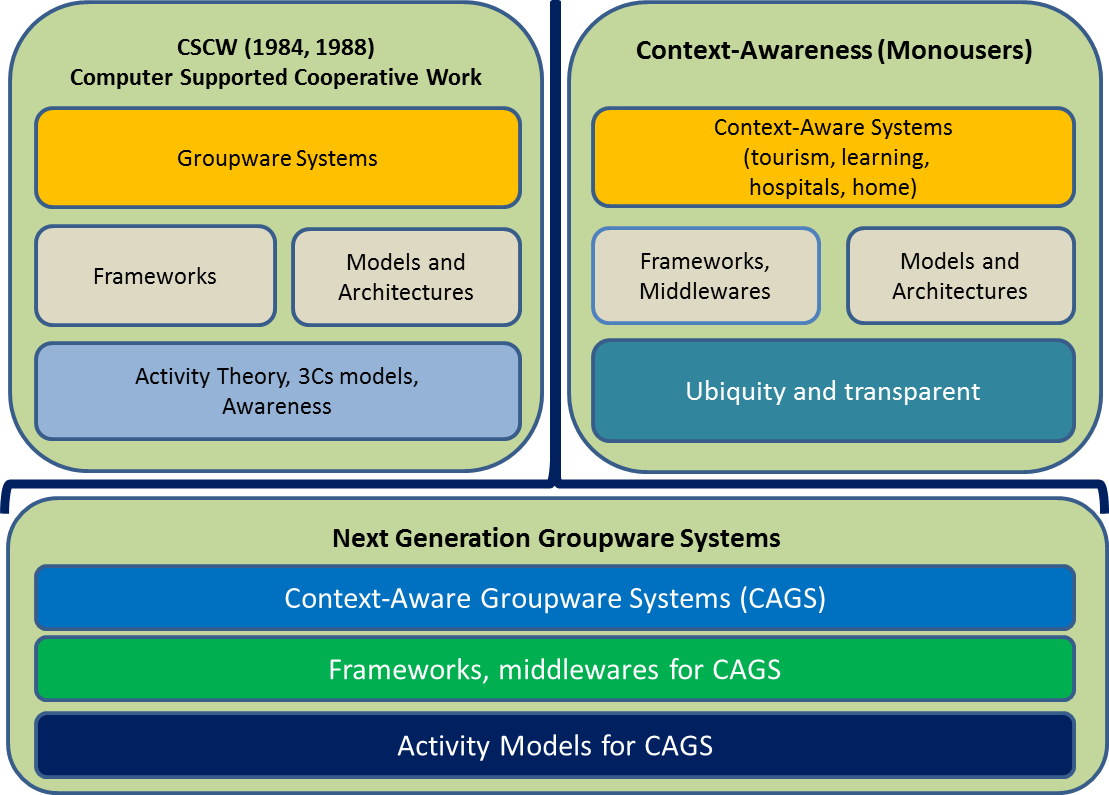
\includegraphics[width=9.4cm]{images/contextoInvestigacion.png}
	\caption{Involved areas in research.} % Áreas involucradas en la investigación
	\label{fig:contextoInvestigacion}
\end{figure}

With the use and development of Groupware, there have emerged classifications that mention that collaboration in work teams can be performed in different circumstances. Table \ref{fig:matrix} shows an instance of the classification proposed on \cite{Johansen88}, it is by time and space, and it incorporates contextual elements, this classification have been useful for the observation and consideration of the types of interactions that happen during the collaboration process. For example, in synchronous distributed interactions, the collaboration might occur in a different place and at the same time, as it happens in collaborative videogames (e.g. Halo, Gears of War, AssaultCube) with audio/video or to the instant messenger tools. However, the means of communication offered by Groupware Systems are not enough for all the cases, particularly we have identified that very often there are situations where communication and coordination tools (e.g. text/audio messages, etc.) are not appropriate to specific collaborative activities, for example, for FPS video game scenario ($s_1$), is not suitable to get coordinated by using instant messages since a player may get distracted while doing this interaction and so he may be terminated. So that it could be recommendable to be able to detect or evaluate certain circumstances in an activity and the users contexts that could be useful for the system, to eventually offer or execute other means of communication or services that are more helpful to the player, and so that the communication or coordination are no longer a distractor for the players.


\begin{figure}[ht!]
	\centering
	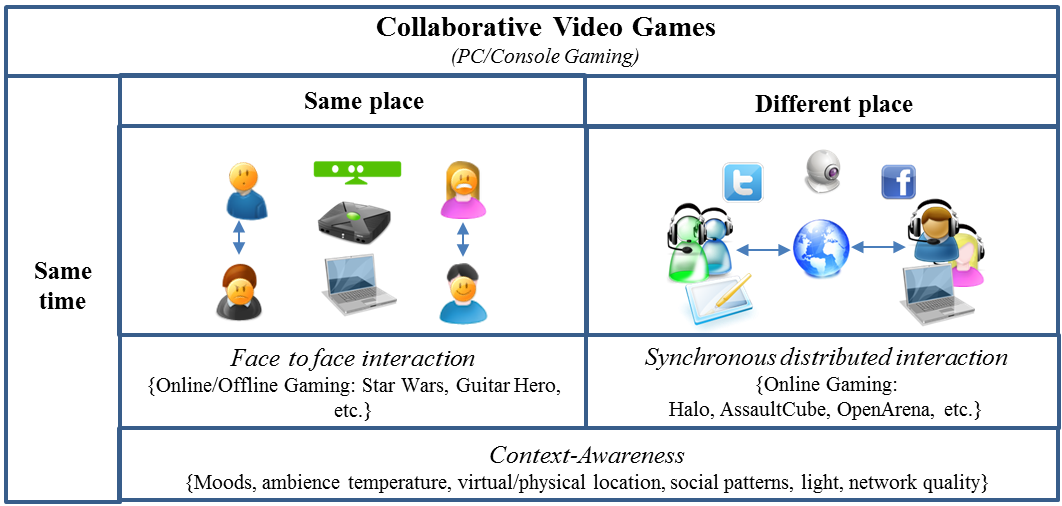
\includegraphics[width=12cm]{images/matrix.png}
	\caption{Matrix of time and space.} % Áreas involucradas en la investigación
	\label{fig:matrix}
\end{figure}

\subsection{Context-Aware Systems}
Nowadays, most of the work related to modeling, management and use of context are intended for systems that do not support collaborative work. These studies have considered variables and user-centered factors such as temperature, time or location, and do not include elements or variables that play an important role at the moment of a social interaction for coordinating, cooperating and communicating, for example, roles, hierarchies, rules, the state of the activity group, other users activities, group planning activities, etc.

There is no definitely interpretation of context, nevertheless, among the most spread definition of context is found that of Dey\cite{Dey01}, who describes it as any information that can be used to represent the situation of an entity. An entity is a person, place or object that is considered relevant between an user and an application, the user and the application itself, so that the context offers a new way to access and provide information and services. Thereby, within the context it is possible to determine information such as the location (GPS), roles, preferences, time, temperatures or activities, and this information allows to the interactions to be performed considering the current status of a user that participates in a collaborative activity. As the context changes quickly, context resources can be obtained by mobile devices, sensors, or personal information provided by software services through the Internet, such as web services or other methods that allow the information exchange.


\subsection{Context-Aware Groupware Systems}

Brezillon et al. \cite{Brezillon08} mention that growth in the areas of i) CSCW and ii) Context-Awareness have largely been independent, which has caused a gap between system designers and researchers of collaborative context awareness. This gap directly affects the building of CAGS that help to increase the information and productivity of the users, although, also it generates an area of opportunity that still needs to be explored.


%\section{Modelos y marcos de trabajo} %Models and frameworks
\section{Context-Aware Collaborative Video Games} %
\label{sec:videogame}
The presence of video games is increasing, this is due largely to the new processing capabilities offered by the devices. It is now possible the innovation of games that use image recognition, geolocation, augmented reality, and other emerging technologies. Although there are solutions or frameworks (e.g. \cite{Diamantaki10,Zea09,Marty11}) that propose alternatives to build such systems, however efforts are limited in collaborative aspects, since do not considered social modeling in complex activities and capture nonverbal information transmitted by users when working. Video games today and collaborative information already consider to measure the performance of users, in order to re-adapt the game and offer a more attractive to them, however, are usually limited to metric measurements as points scored above or game levels which has unlocked. For this reason it is attractive to propose a new model that considers elements with a higher incidence in the collaboration of users, for sample,  considering variables as such roles to play, group rules, information received verbal or nonverbal, goals, unusual behaviors, objects manipulated, social protocols, communication used (e.g. visual, physical), actions (e.g. write, speak, etc.). The analysis in the current literature has led to the identification and grouping of important aspects to consider in business models. The proposed approaches raise partial solutions (e.g. models, architectures, platforms) that help in building CAGS systems, and this has been a first approach to propose a model of collaboration.


\begin{figure}[ht!]
	\centering
			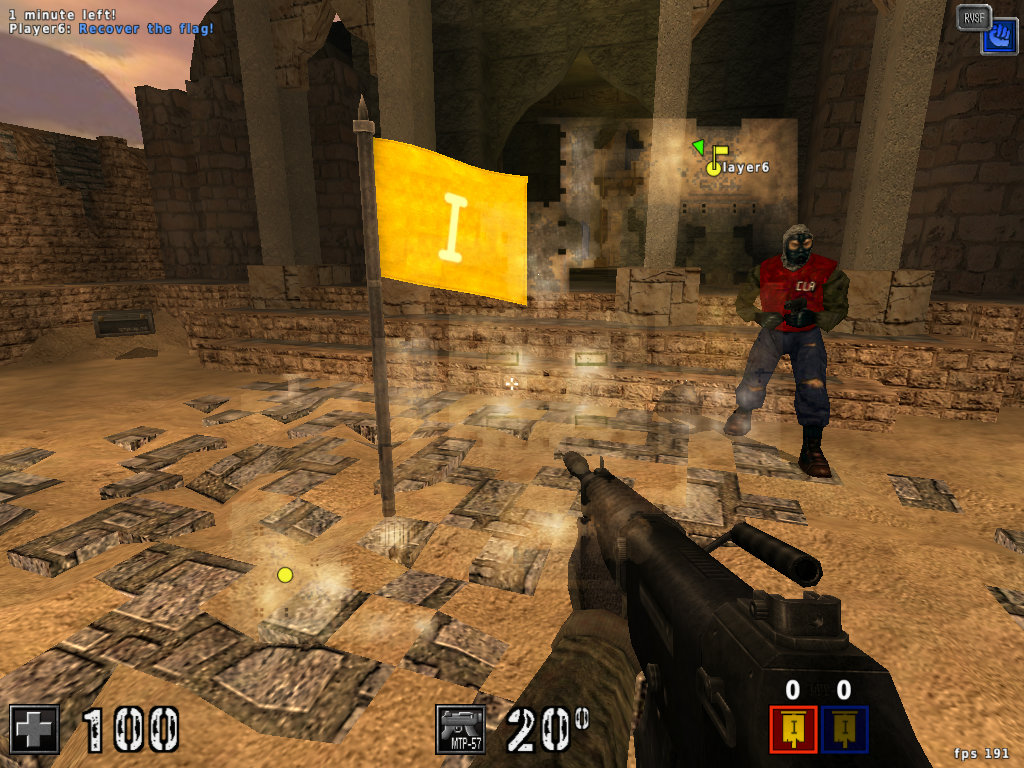
\includegraphics[width=8.7cm,height=5cm]{images/juego.jpg}
	\caption{Video Game screen with location map and the flag.}
	\label{fig:juego}
\end{figure}


\section{Experimental Study} 
\label{sec:study}

For both cases $e_1$ and $e_2$, a subjective instrument to measure user satisfaction was conducted with Likert scale (see \ref{tab:RelationOfStatementsInTheSurvey}). The instrument consists of 12 questions that refer to 6 dimensions related to user satisfaction, such as (D1) Coordination (1-2), (D2) Communication (3-4), (D3) Cooperation (5-6), (D4) Entertaining (7-8), (D5) Ease (9-10) and (D4) Awareness (11-12). The used scale for responses for a range of 1-5, where ``1'' stands for Strongly Disagree, ``2'' for Disagree, ``3'' Neither agree nor disagree, ``4'' Agree and ``5'' Strongly Agree. To validate the consistency of the evaluation instrument, was applied Cronbach Alpha coefficient to data obtained with the players of $e_1$, the coefficient was applied to each dimension of the scale and the results were as follows: D1 = 0.7, D2 = 0.5, D3 = 0.6, D4 = 0.8, D5 = 0.5 and D6 = 0.5, as can be seen, in D1, D3 and D4 the values are equal to or greater than 0.6, therefore, the questions in these dimensions have reliability moderate/acceptable. In D2, D5 and D6 did not reach a value of 0.6 or higher, however, the obtained data were not significant to discard these items. In addition, the average of all the dimensions was 0.6, which is considered moderately acceptable. However, we expected to improve the items for future applications (D2, D5 and D6) and increase the sample size.

\begin{table}[htbp]
\renewcommand{\arraystretch}{1.2}
%\normalsize
	\centering
		\begin{tabular}{|l|l|l|}
			\hline
		 	\head{No.} & \head{Dimension}	& \head{Statement} \\
			\hline
			1&D1&Text messages offered by the game were helpful to organize with\\
			& & your teammates. \\ \hline 
			2&D1&Location map in the game helped you generate an estrategy with \\
			&&your other teammates. \\  \hline
			3&D2&Audio messages predefined in the game were enough to transmit \\ 
			&&your emotions in the game. \\  \hline
			4&D2&Text messages were useful for transmiting information to your \\
			&&teammates during collaborative activity. \\  \hline
			5&D3&Location map of your teammates is useful to support the group \\
			&& activity. \\ \hline
			6&D3&The video game offers suitable collaboration tools to help your \\
			&&team. \\ \hline 
			7&D4&The video game kept you entertained for the development of the \\
			&&game. \\\hline 
			8&D4&Information (e.g. messages, alerts, etc.) shown on the game  \\
			&&interface possively affect your entertainment. \\ \hline 
			9&D5&The video game is easy to use in order to collaborate with your \\
			&&teammates. \\ \hline
			10&D5&The video game is easy to use in order to remove players from \\ 
			&&the contrary team. \\  \hline
			11&D6&Knowing the location of your teammates on the map helped your \\
			&&activity in the game. \\ \hline 
			12&D6&Knowing the score of all the players positively changed your \\
			&&behavior during the collaborative activity. \\ \hline
		\end{tabular}
	\caption{Relation of statements in the survey.}
	\label{tab:RelationOfStatementsInTheSurvey}
\end{table}


\subsection{Results}
\label{sec:results}

\section{Discussion}
\label{sec:discussion}
The results obtained with the Likert instrument in $e_1$ and $e_2$ has been opposite referring to collaboration mechanisms (D1, D2, D3), this retrieve us evidence that the traditional mechanisms offered in the FPS video games are not sufficient and not presented in the best way, therefore, it is interesting to propose better tools that include contextual information to make more efficient collaboration. Finally, the evaluation also helped us identify social behaviors that could be studied in greater depth, for example, natural setting roles, identification of moods, detection of patterns generated by the groups, recognition of social interactions, to name few.

Table \ref{tab:faceToFaceIndicators} shows the events found in the observation of the collaborative videogame, particularly were presented in face-to-face case, but could not be transmitted or received in the distributed case, using computer-mediated interactions.

\begin{table}[htbp]
%\renewcommand{\arraystretch}{1.2}
%\normalsize
	\centering
	\begin{tabular}{ll}
			\hline
		 	Category & Events \\
			\hline
			 Affective & Cultural identification, emotions or direct expressions \\
			 & of moods (laughter, gestures). \\
			 Interactive & Transparency and naturalness in the interactions, \\
			 & assigning roles, modification and creation of artifacts or \\
			 & objects. \\
			 Cohesive & Trust generated by contact auditory/visual /verbal, \\
			 & perception of skills (leadership, roles), \\
		   & evolution of social identities (partnerships) \\
			\hline	 
	\end{tabular}
	\caption{Observed elements in exploratory study.}
	\label{tab:faceToFaceIndicators}
\end{table}


\section{Conclusions and Future Work}
\label{sec:conclusion}
This paper presents a study where is described the areas that are directly involved in the construction of Context-Aware Groupware Systems (CAGS). From the CSCW and contextual awareness, this work introduces collaboration in terms of cooperation, coordination and communication. Also, one exploratory study was carried out in order to observe the behavior of users in a collaborative activity on a First-Person Shooter (FPS) video game, the purpose of this study was to identify elements and conditions that may be explored in future studies, mainly to improve traditional means of communication offered in this type of applications. As well, to streamline the means of communication, is not intended to make easier the game's plot, but the to provide mechanisms to improve the experience of users when using collaborative tools offered in the game. This is expected to include contextual information of the players and the interactions of activities, for example, for future stages, our interest is that the game automatically provide appropriate means of collaboration (e.g. messages) depending on the executed interaction (e.g. player captures the flag on the battlefield), without requiring the user to explicitly invoke these tools, since as mentioned earlier in the game occurred many cases where users were destroyed by distracted when explicitly invoked and write messages text or audio.

% use section* for acknowledgement
%\section*{Acknowledgment}
%Este trabajo es parte de un proyecto de investigación ``...'' por Conacyt y la Universidad Veracruzana.

% references section
\bibliographystyle{./bibtex/splncs03}
\bibliography{./bib/paper}
\end{document}
